\section{GPU Vector Join}\label{sec:motivation}

% define vector join and its three modes
A \emph{vector join} is a similarity join between two relations of embeddings that runs inside a SQL engine.
It is the join of the third stage in Section~\ref{subsec:vector-join}, and we use this term for the rest of the paper.
Its three forms are its \emph{modes}: per-row top-$k$, global top-$k$, and threshold.
A batched vector search is itself a per-row top-$k$ vector join (Section~\ref{subsec:gpu-data-processing}).

% workloads that are vector joins, and the mode each one uses
The workloads for the vector join already exist under different names.
In machine learning pipelines, semantic deduplication joins a training corpus against itself to find and remove near-duplicate data points, and pruning this redundancy has been shown to improve both data efficiency and downstream model quality~\cite{HuSieveIVF26, AbbasSemDeDup23}.
In data integration, entity resolution matches records across two sources by the similarity of their learned embeddings, which reduces a classically hard matching problem to a similarity join~\cite{SantanaEMJoin25, SantanaRibeiro23}.
In retrieval and recommendation, a batch of user or query embeddings is compared against an item catalog or document corpus at once for offline candidate generation, evaluation, or the mining of hard negatives that train the next embedding model~\cite{HuangFBRetrieval20, XiongANCE21, ThakurBEIR21}.
The per-row top-$k$ mode serves workloads that need the nearest neighbors of every probe row, such as batch retrieval and hard-negative mining, and the threshold mode serves workloads that need every pair within a distance bound, such as deduplication and entity resolution.

\subsection{The Transition: From Vector Search to Vector Join}\label{subsec:the-transition}

%\yxy{add more details to the figure to make it more interesting, like example systems (only the most important ones)}}
% new feedback, make it more colorful, instead of showing example systems, show a short description
\begin{figure}
    \centering
    \begin{tikzpicture}[
        font=\small\sffamily,
        cell/.style={draw, rounded corners=2pt, minimum width=2.5cm,
        minimum height=1.4cm, align=center,
        font=\small\sffamily\bfseries},
        open/.style={cell, dashed, line width=0.9pt, fill=black!8},
        ax/.style={font=\small\sffamily\bfseries, align=center},
        flow/.style={-{Latex[length=2.2mm]}, thick, black!65},
    ]

        % columns: relational, vector; rows: OLTP, CPU OLAP, GPU OLAP
        \node[cell] (r1) at (0,0)      {70s--80s\\[2pt] {\scriptsize\mdseries Oracle, PostgreSQL,}\\ {\scriptsize\mdseries MySQL, SQL Server}};
        \node[cell] (r2) at (0,-2.5)   {$\sim$mid-1990s\\[2pt] {\scriptsize\mdseries Snowflake, BigQuery,}\\ {\scriptsize\mdseries Databricks, DuckDB}};
        \node[cell] (r3) at (0,-5.0)   {2010s\\[2pt] {\scriptsize\mdseries Sirius, Theseus,}\\ {\scriptsize\mdseries HeavyDB, Kinetica}};
        \node[cell] (v1) at (4.5,0)    {late 2010s\\[2pt] {\scriptsize\mdseries Milvus, Pinecone,}\\ {\scriptsize\mdseries pgvector, Oracle}};
        \node[cell] (v2) at (4.5,-2.5) {2024\\[2pt] {\scriptsize\mdseries Databricks, Spark,}\\ {\scriptsize\mdseries BigQuery, DuckDB}};
        \node[open] (v3) at (4.5,-5.0) {this work\\[2pt] {\scriptsize\mdseries Sirius}};

        % arrows
        \draw[flow] (r1) -- node[fill=white, inner sep=1pt, font=\scriptsize\sffamily\mdseries, align=center] {data warehousing,\\column stores} (r2);
        \draw[flow] (r2) -- node[fill=white, inner sep=1pt, font=\scriptsize\sffamily\mdseries, align=center] {memory bandwidth,\\cost efficiency} (r3);
        \draw[flow] (v1) -- node[fill=white, inner sep=1pt, font=\scriptsize\sffamily\mdseries] {batch ML workloads} (v2);
        \draw[flow] (v2) -- node[fill=white, inner sep=1pt, font=\scriptsize\sffamily\mdseries] {compute throughput} (v3);
        \draw[flow] (r1) -- node[above, font=\scriptsize\sffamily\mdseries, align=center] {embedding\\models} (v1);
        \draw[flow] (r3) -- node[above, font=\scriptsize\sffamily\mdseries, align=center] {embeddings in\\the warehouse} (v3);

        % column axis (x)
        \node[ax, anchor=south] at ([yshift=3pt]r1.north) {Relational};
        \node[ax, anchor=south] at ([yshift=3pt]v1.north) {Vector};

        % row axis (y)
        \node[ax, anchor=east, inner xsep=0pt] at ([xshift=-6pt]r1.west) {OLTP};
        \node[ax, anchor=east, inner xsep=0pt] at ([xshift=-6pt]r2.west) {CPU\\OLAP};
        \node[ax, anchor=east, inner xsep=0pt] at ([xshift=-6pt]r3.west) {GPU\\OLAP};
    \end{tikzpicture}
    \caption{
        Each cell shows when the transition began and its representative systems (not necessarily from that period), and arrows label what drove it. Relational data moved from transactional to analytical processing on CPUs~\cite{StonebrakerPavloAround24}, then to GPUs~\cite{AramburuTheseus25, HeavyDB, Kinetica, Yogatama26}. Vector data is following the same path: vector search serves point queries~\cite{StonebrakerPavloAround24, WangMilvus21}, and the vector join is now a SQL clause in several CPU engines~\cite{DuckDBVSSBlog24, DatabricksNearestByJoinBlog26, DuckDBNearestByPR24137, SparkNearestByJoin26}. The vector join on the GPU is the open cell that this work fills.
    }
    \label{fig:quadrant}
\end{figure}


% Figure 1, relational side: OLTP and OLAP are different problems with different engines
Relational workloads split into transaction processing (OLTP) and analytical processing (OLAP) because the two turned out to be different problems~\cite{StonebrakerPavloAround24}.
An OLTP query asks ``what matches this'' and looks up one customer, one order, or one account, while an OLAP query asks ``what matches what'' and joins whole tables against each other.
OLTP serves lookups from persistent indexes built ahead of time (e.g., B-trees) and is measured by latency, while OLAP builds temporary structures (e.g., a hash table) at query time over intermediate results, and is measured by throughput.
Stonebraker and \c{C}etintemel argued that these differences end the era of a single general-purpose engine~\cite{StonebrakerOneSize05}, and column stores such as C-Store and MonetDB proved this in practice~\cite{StonebrakerCStore05, IdreosMonetDB12}.
These engines now form the basis of decision support over historical data~\cite{ChaudhuriDayal97}.
We argue that vector data is now at the same transition point (Figure~\ref{fig:quadrant}).

% Figure 1, vector side: vector search is the OLTP half, and the vector join is the OLAP half
Vector search is the OLTP half: it asks ``what is similar to this'' and returns the nearest neighbors of one query vector.
The vector join is the OLAP half: it asks ``what is similar to what'' and relates the rows of one table of vectors to the rows of another.
A relational join follows relationships that were declared ahead of time as keys, while a vector join finds relationships that nobody declared, between rows that share no key but a meaning.
We believe the vector join can play the same role in decision support for everything that embeddings make comparable.

\subsection{The Vector Join as a GPU Database Operator}\label{subsec:why-gpu-database}

% moved from old Sec 4:
% \andy{i think we should also mention that none of the gpu libraries provide a threshold API, while the workload already exist, and we should argue that the type of join we do is about the same, it's just the reduction phase that need to vary (so this becomes are 3rd arg) ... or maybe not because threshold is a different kernel -> move this to new 3.2}

% the vector join is a matrix product, so its work is dominated by GEMM
The vector join is an especially good fit for the GPU, because moving from one query vector to many changes the kind of work the hardware does.
Under the metrics of Section~\ref{subsec:embeddings-and-vectors}, for two vectors $r$ and $s$, their inner product is $r \cdot s$, cosine similarity divides it by $\lVert r \rVert \lVert s \rVert$, and squared L2 distance expands to $\lVert r \rVert^2 + \lVert s \rVert^2 - 2\, r \cdot s$.
If the probe vectors are stacked as the rows of an $m \times d$ matrix $R$ and the corpus vectors as the rows of an $n \times d$ matrix $S$, all $mn$ dot products are the entries of the matrix product $RS^\top$.
The norms take $O((m+n)d)$ work and are computed once per vector, while the product takes $O(mnd)$ and is computed once per pair, so when both sides are large, the work is dominated by a dense matrix multiplication (GEMM).
Columnar engines store a column of embeddings as one contiguous matrix, and the GPU is built to compare one matrix against another.

% a search is bandwidth-bound and a join is compute-bound, so the join belongs in a GPU-native SQL engine
A single search ($m=1$) is a matrix-vector product, in which each corpus vector is read once and used once, so it is bound by memory bandwidth and leaves most of the GPU's compute idle.
For a join, $RS^\top$ is a matrix-matrix product in which each corpus vector is reused across many probe rows, so the work becomes compute-bound and runs as GEMM.
Without this reuse, computing distances one pair at a time reads two values for every multiply-accumulate (MAC), so it is bound by memory bandwidth as well.
% \andy{explains MACs = distance computations × d in evaluation}
To make the join compute-bound, the Databricks operator reuses each corpus vector across a tile of probe rows, and their roofline estimate shows that this holds once about 64 query vectors are buffered~\cite{DatabricksNearestByJoinBlog26}.
Once the join is compute-bound, its speed depends on how much arithmetic the hardware delivers.
We therefore argue that the vector join should run as an operator in a GPU-native SQL engine.

\begin{figure}[t]
    \centering
    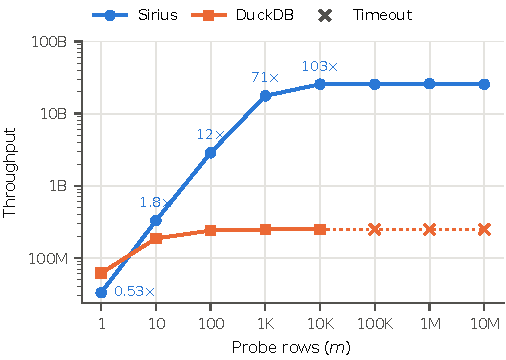
\includegraphics[width=0.8\columnwidth]{exact-probe-sweep}
    \captionsetup{textfont=normalfont}
    \caption{Exact threshold join against SIFT10M with tables in memory.}
    \label{fig:exact-probe-sweep}
\end{figure}


% evidence: the GPU's advantage grows as the probe side grows
\andy{TODO: revisit this, need a new run after the code change, or maybe move get rid of this paragraph and point to evaluation}
Our measurements in the exact setting show that the GPU's advantage grows as the work moves from a matrix-vector product to a matrix-matrix product (Figure~\ref{fig:exact-probe-sweep}).
We run an exact threshold join against Bigann10M and vary the number of probe rows $m$ from one to 10M\@.
At $m=1$, Sirius is ....
As $m$ grows, Sirius's throughput rises ..., while DuckDB's plateaus at about 250 million by $m=100$.
